
\documentclass{beamer}

\mode<presentation> {
% The Beamer class comes with a number of default slide themes
% which change the colors and layouts of slides. Below this is a list
% of all the themes, uncomment each in turn to see what they look like.

%\usetheme{default}
%\usetheme{AnnArbor}
%\usetheme{Antibes}
%\usetheme{Bergen}
%\usetheme{Berkeley}
%\usetheme{Berlin}
%\usetheme{Boadilla}
%\usetheme{CambridgeUS}
%\usetheme{Copenhagen}
%\usetheme{Darmstadt}
%\usetheme{Dresden}
%\usetheme{Frankfurt}
%\usetheme{Goettingen}
%\usetheme{Hannover}
%\usetheme{Ilmenau}
%\usetheme{JuanLesPins}
%\usetheme{Luebeck}
\usetheme{Madrid}
%\usetheme{Malmoe}
%\usetheme{Marburg}
%\usetheme{Montpellier}
%\usetheme{PaloAlto}
%\usetheme{Pittsburgh}
%\usetheme{Rochester}
%\usetheme{Singapore}
%\usetheme{Szeged}
%\usetheme{Warsaw}

% As well as themes, the Beamer class has a number of color themes
% for any slide theme. Uncomment each of these in turn to see how it
% changes the colors of your current slide theme.

%\usecolortheme{albatross}
%\usecolortheme{beaver}
%\usecolortheme{beetle}
%\usecolortheme{crane}
%\usecolortheme{dolphin}
%\usecolortheme{dove}
%\usecolortheme{fly}
%\usecolortheme{lily}
%\usecolortheme{orchid}
%\usecolortheme{rose}
%\usecolortheme{seagull}
%\usecolortheme{seahorse}
%\usecolortheme{whale}
%\usecolortheme{wolverine}

%\setbeamertemplate{footline} % To remove the footer line in all slides uncomment this line
%\setbeamertemplate{footline}[page number] % To replace the footer line in all slides with a simple slide count uncomment this line

%\setbeamertemplate{navigation symbols}{} % To remove the navigation symbols from the bottom of all slides uncomment this line
}
\usepackage[backend=biber]{biblatex}
\bibliography{reference.bib} 
\usepackage{multirow}
\usepackage{hhline}
\usepackage{fec}
\usepackage{subfigure}
\usepackage{graphicx} % Allows including images
\usepackage{booktabs} % Allows the use of \toprule, \midrule and \bottomrule in tables
\usepackage{array}
\usepackage{graphicx}
\usepackage{lscape}
\usepackage{verbatim}
\usepackage{amsmath}
\usepackage{mathtools}
\DeclarePairedDelimiter{\norm}{\lVert}{\rVert} 
\setbeamertemplate{theorems}[numbered] 
\newtheorem{remark}{Remark} %for remark 
%----------------------------------------------------------------------------------------
%	TITLE PAGE
%----------------------------------------------------------------------------------------

\title[Short title]{Complexity of Pivot Algorithms} % The short title appears at the bottom of every slide, the full title is only on the title page

\author{Qi Wang, Sean Kelley} % Your name
\date{\today} % Date, can be changed to a custom date

\begin{document}

\begin{frame}
\titlepage % Print the title page as the first slide
\end{frame}

\begin{frame}
\frametitle{Overview} % Table of contents slide, comment this block out to remove it
\tableofcontents % Throughout your presentation, if you choose to use \section{} and \subsection{} commands, these will automatically be printed on this slide as an overview of your presentation
\end{frame}

%----------------------------------------------------------------------------------------
%	PRESENTATION SLIDES
%----------------------------------------------------------------------------------------

%------------------------------------------------
\section{Pivot Rules} % Sections can be created in order to organize your presentation into discrete blocks, all sections and subsections are automatically printed in the table of contents as an overview of the talk
%------------------------------------------------
\begin{frame}
\frametitle{Other Pivot Rules}
\begin{itemize}
\item Best improvement rule: choose entering $j := \arg \max_{j\in N}(c_B^T A_B^{-1} A_j - c_j)\times t_j$ where $t_j = \min_{i \in \{B:(A_B^{-1}A_j)_{i} >0\}} \frac{x_i}{(A_B^{-1}A_j)_{i}}$
\item Steepest edge rule: choose entering $j: = \arg\max_{j \in N} \frac{c_B^TA_B^{-1}A_j - c_j}{\norm{A_B^{-1}A_j}}$
\item Last-in-first-out rule (LIFO): choose the most recently moved variable.
\item Most-often-selected-variable (MOSV): choose the variable that has been selected the largest amount of times before.
\end{itemize}
\end{frame}

%------------------------------------------------
\subsection{S-monotone index selection rules}
\begin{frame}
\frametitle{S-monotone index selection rules\cite{csizmadia2012s}}
What is \textbf{s}?

- At iteration $k$, $s_k \in \Nmbb^{n}$. Generate $s_k$ at each iteration. And choose the candidate of entering basis indices $j := \arg \max_j {s_k^j}$.

How to generate $s_k$?

\begin{itemize}
\item Bland's rule: $s_k = (n, n-1, \cdots, 1)^T$ for all $k$.
\item LIFO. \begin{align*}
s_{k+1}^i = \left\{
\begin{aligned}
&k, & \text{if } i \in \{i_k, o_k\},\\
&s_k^i & \text{ otherwise}. 
\end{aligned}
\right.
\end{align*}
\item MOSV. \begin{align*}
s_{k+1}^i = \left\{
\begin{aligned}
&s_k^{i} + 1, & \text{if } i \in \{i_k, o_k\},\\
&s_k^i & \text{ otherwise}. 
\end{aligned}
\right.
\end{align*}
\end{itemize}
\end{frame}

\begin{frame}[allowframebreaks]
\frametitle{S-monotone index selection rules}
What is "s-monotone"?

- For iteration $k-1$ and $k$, $s_{k-1}^i \le s_{k}^i$ for all $i= 1,\cdots, n$.
\begin{theorem}
The simplex algorithms and the criss-cross algorithm with s-monotone index selection rules are finite for linear programming problems.
\end{theorem}
\framebreak
Revise steepest-edge rule to be s-monotone version.
\begin{enumerate}
\item At the beginning, define a strictly increasing sequence $\{p_k\}$.
\item At iteration $k$, let
$$
\gamma = \max_{j \in N} \frac{c_{B^k}^TA_{B^k}^{-1}A_j - c_j}{\norm{A_{B^k}^{-1}A_j}},
$$
and adjust $p_k$ by
 \begin{align*}
p_k = \left\{
\begin{aligned}
&p_k + \delta, & \text{if } p_{k-1} \ge \gamma,\\
&\gamma, & \text{ otherwise}. 
\end{aligned}
\right.
\end{align*}
where $\delta > 0$ is a given number. 
\item Update the $s_{k}$ as
\begin{align*}
s_{k}^i = \left\{
\begin{aligned}
&p_k, & \text{if } i \in \{i_k, o_k\},\\
&s_{k-1}^i & \text{ otherwise}. 
\end{aligned}
\right.
\end{align*}
\end{enumerate}
\end{frame}



%------------------------------------------------
\section{Complexity Analysis}
%-----------------------------------------------
\subsection{Worst Case - Klee Minty Cube}
\begin{frame}
\frametitle{Worst Case - Klee Minty Cube}
Klee-Minty Cube LO problem
\begin{align*}
\begin{split}
\max &\sum_{j=1}^n 2^{n-j}x_j \\
\text{s.t. } & 2\sum_{j=1}^{i-1}2^{i-j}x_j + x_i \le 5^i, \quad i=1,\cdots,n\\
			&x_j \ge 0,  \quad j=1,\cdots,n
\end{split}
\end{align*} 
Primal simplex with Dantzig's rule may visit all vertices before finally finding the optimal solution ($2^n - 1$ iterations).
\end{frame}


\begin{frame}
\frametitle{Worst Case - Klee Minty Cube}
Klee-Minty Cube LO problem ($n=2$ and $n=3$)
\begin{align*}
\begin{split}
\max \quad & 2x_1 + x_2 \\
\text{s.t. }\quad  & x_1 \le 5\\
& 4x_1 + x_2 \le 25\\
& x_1 \ge 0,\ x_2 \ge 0.
\end{split}
\begin{split}
\max \quad & 4x_1 + 2x_2 + x_3 \\
\text{s.t. }\quad  & x_1 \le 5\\
& 4x_1 + x_2 \le 25\\
& 8x_1 + 4x_2 + x_3 \le 125\\
& x_1 \ge 0,\ x_2 \ge 0, \ x_3 \ge 0.
\end{split}
\end{align*}
\begin{figure}
    \subfigure[]{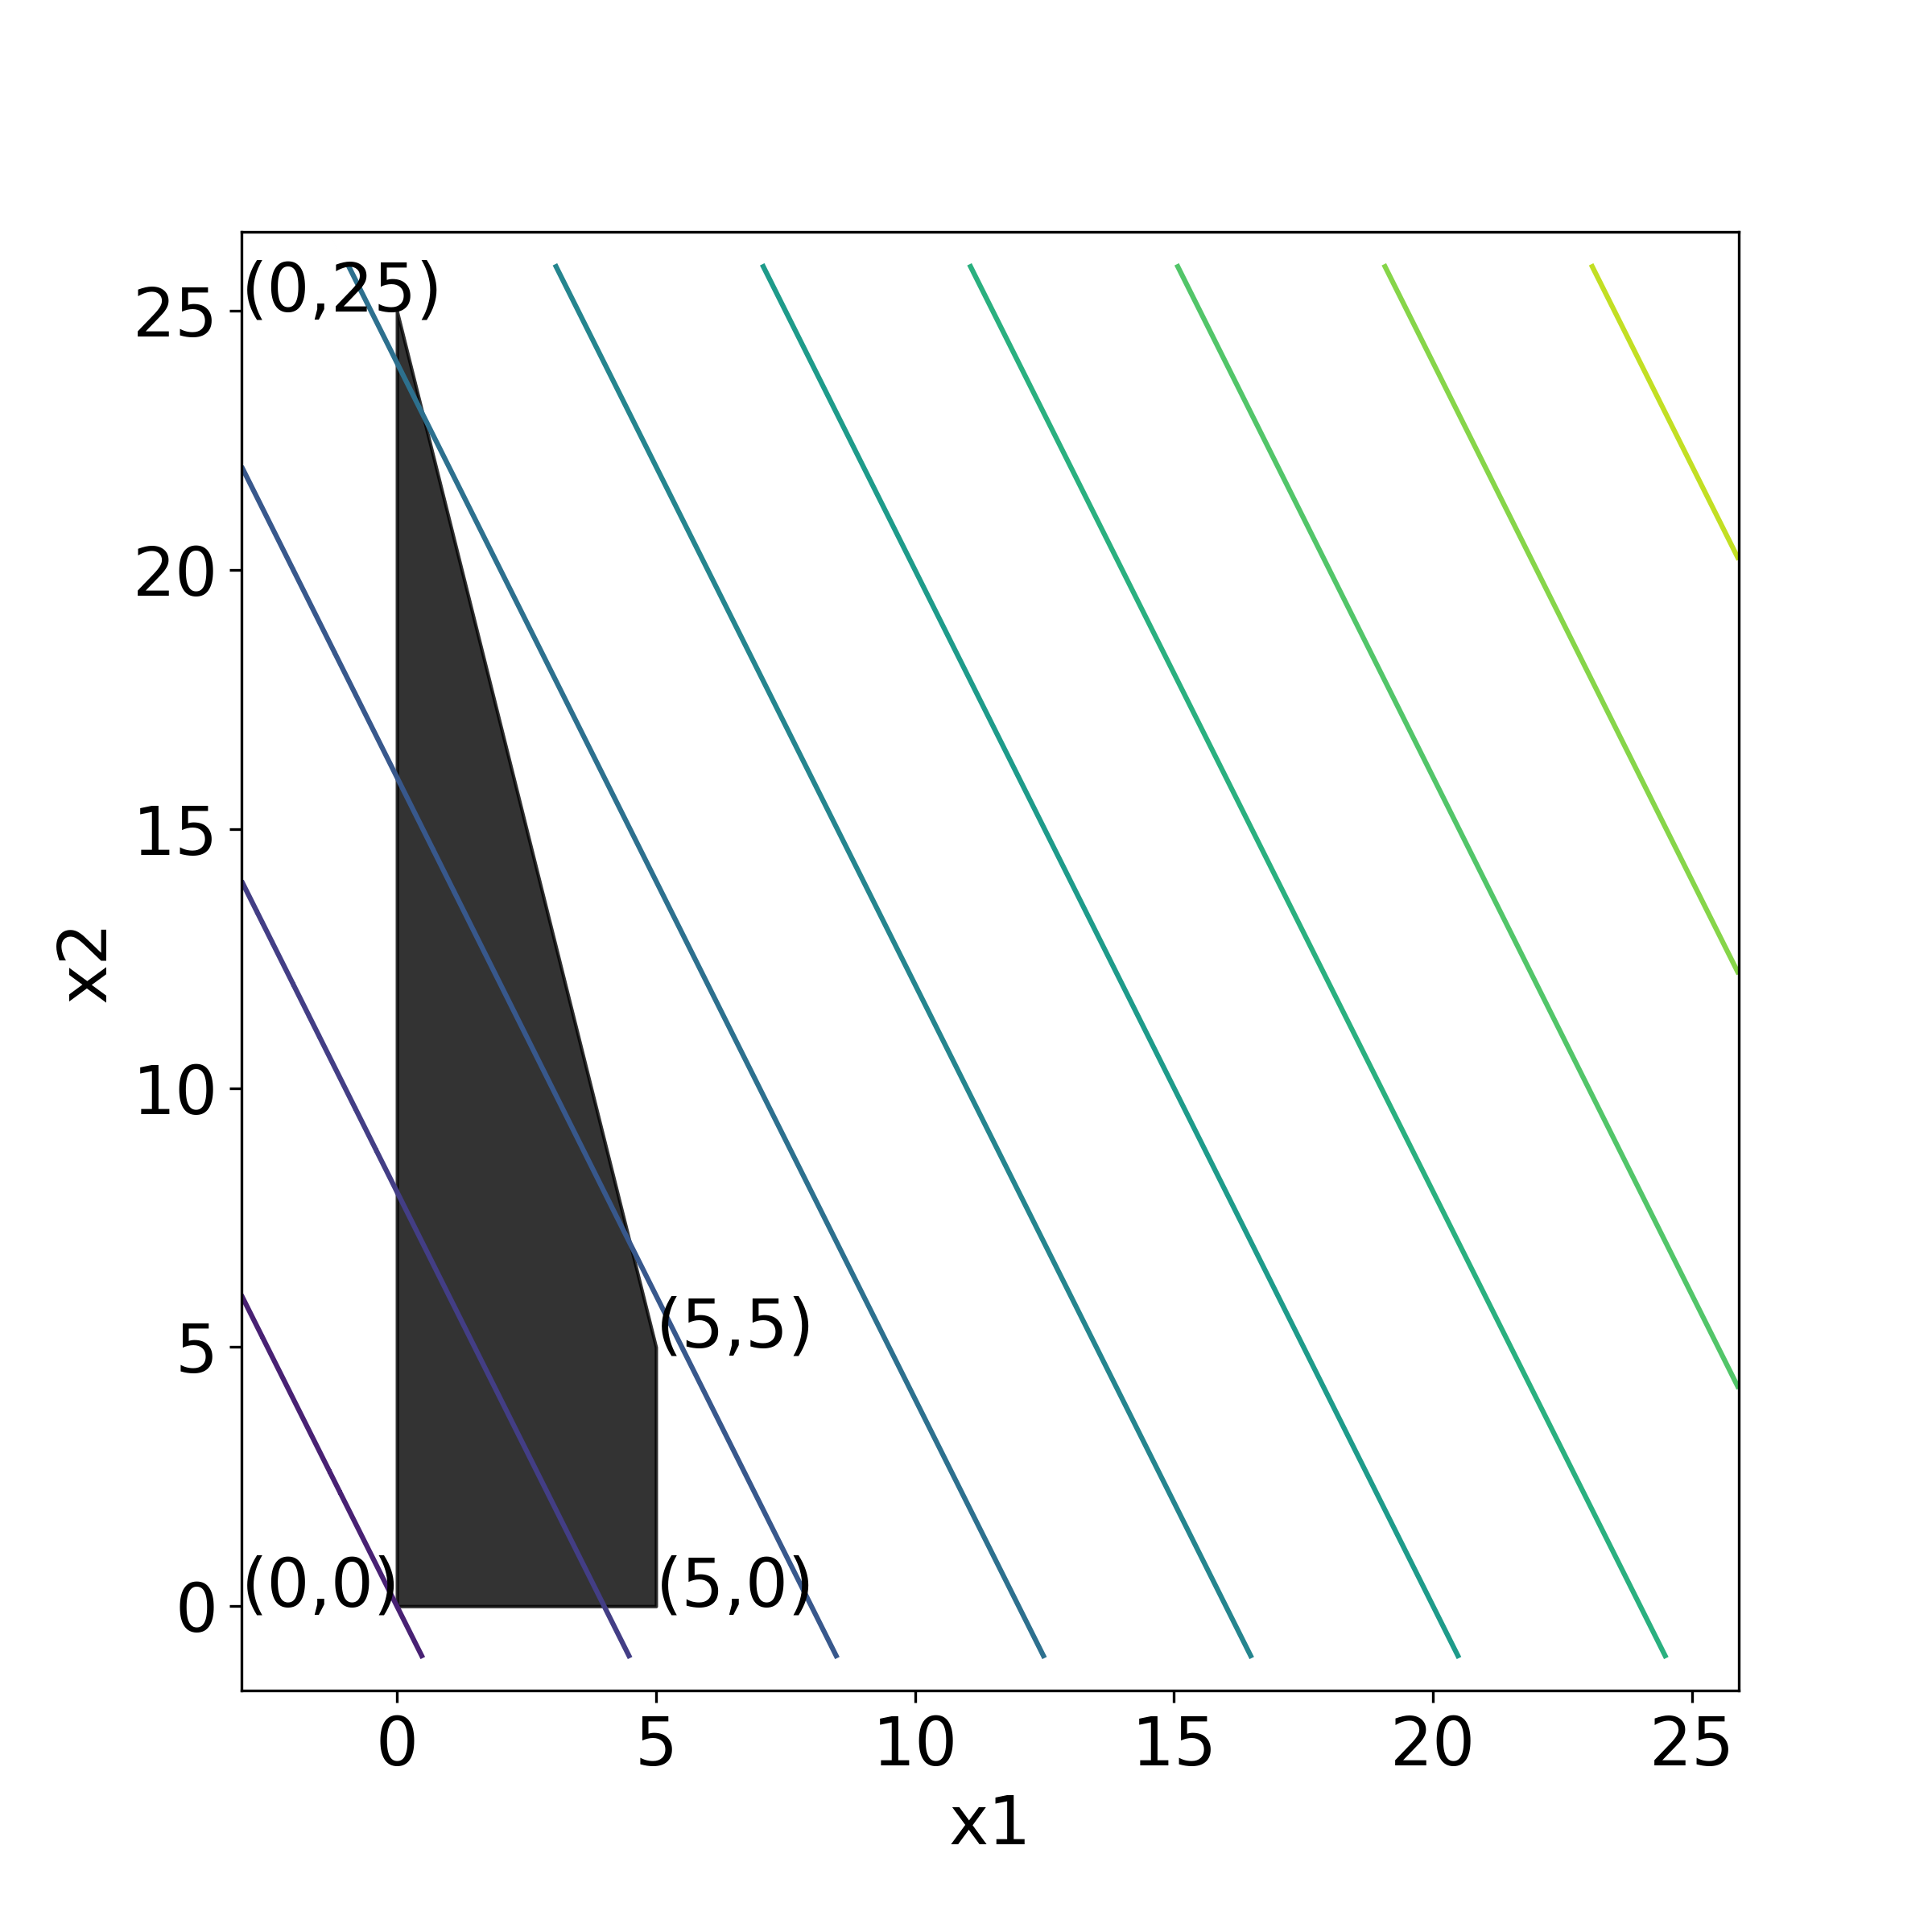
\includegraphics[width=0.35\textwidth]{klee_cube_d2.png}}
    \subfigure[]{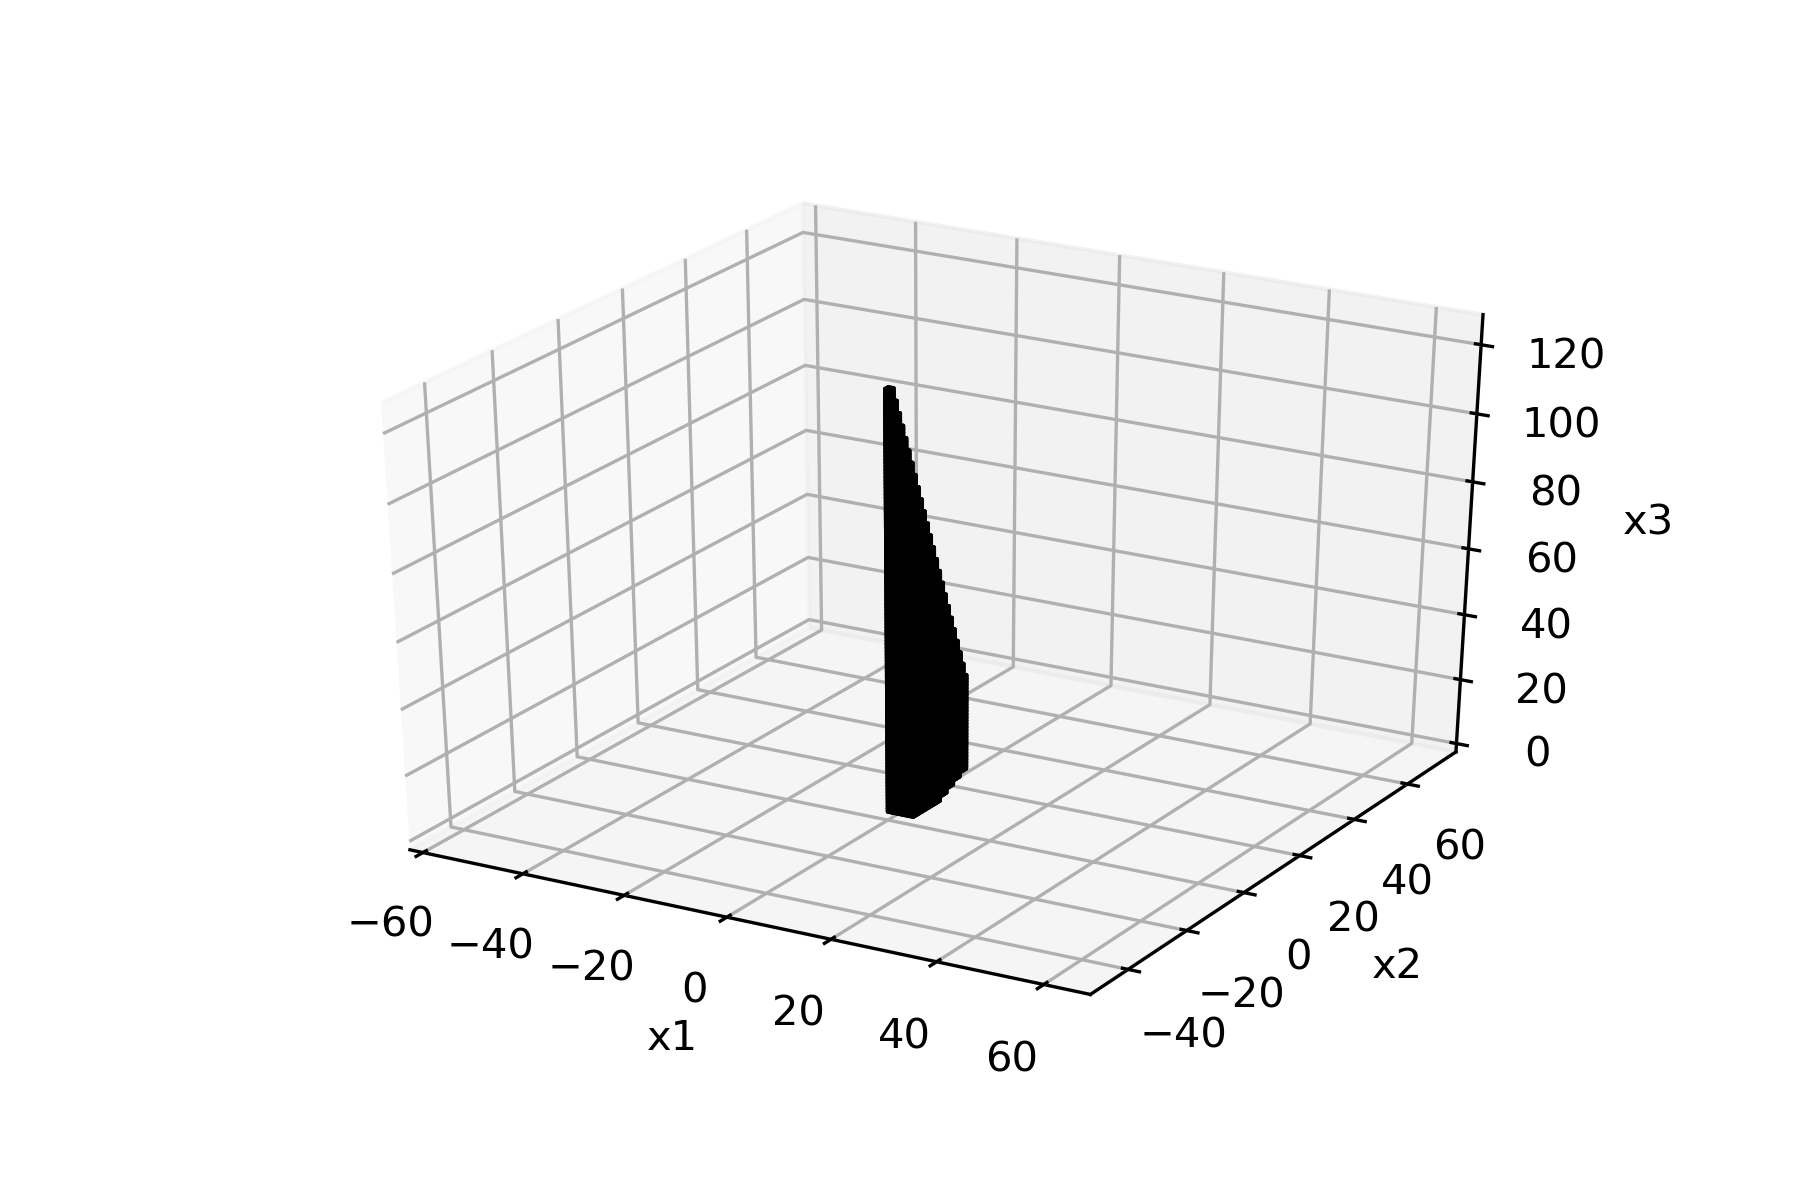
\includegraphics[width=0.55\textwidth]{klee_cube_d3.png}}
\end{figure}

\end{frame}

\begin{frame}{Solving 2-d Klee Minty Cube using Simplex method with Dantzig's rule}
\centering
\begin{tabular}{c|llllll}
   & rhs & $x_1$ & $x_2$ & $s_1$ & $s_2$ &                 \\ \cline{1-6}
$z$  & 0   & 2  & 1  & 0  & 0  & at vetex (0,0), $x_1$ enter, $s_1$ leave  \\
$s_1$ & 5   & $1^*$  & 0  & 1  & 0  &                 \\
$s_2$ & 25  & 4  & 1  & 0  & 1  &                 \\ \hhline{======}
$z$  & -10 & 0  & 1  & -2 & 0  & at vetex (5,0), $x_2$ enter, $s_2$ leave  \\
$x_1$ & 5   & 1  & 0  & 1  & 0  &                 \\
$s_2$ & 5   & 0  & $1^*$  & -4 & 1  &                 \\ \hhline{======}
$z$  & -15 & 0  & 0  & 2  & -1 & at vetex (5,5),  $s_1$ enter, $x_1$ leave \\
$x_1$ & 5   & 1  & 0  & $1^*$  & 0  &                 \\
$x_2$ & 5   & 0  & 1  & -4 & 1  &                 \\ \hhline{======}
$z$  & -25 & -2 & 0  & 0  & -1 & at vetex (0,25), optimal \\
$s_1$ & 5   & 1  & 0  & 1  & 0  &                 \\
$x_2$ & 25  & 4  & 1  & 0  & 1  &                 \\ \hhline{======}
\end{tabular}
\end{frame}


%------------------------------------------------
\subsection{Kitahara and Mizuno Analysis}
\begin{frame}
\frametitle{Kitahara and Mizuno Analysis\cite{kitahara2013bound}}
Notations: 
\begin{itemize}
\item BFS: a basic feasible solution for primal standard LO problem.
\item $\delta$ and $\gamma$: the minimum and the maximum values of all the positive elements of all BFSs. That is, for any BFS $\hat{x} \in \Rmbb^{n}$, if $\hat{x}_j \neq 0, \ j \in \{1, \cdots, n\}$ where $j$ represents the $j$th entry of $\hat{x}$, we have 
\begin{align*}
\delta \le \hat{x}_j \le \gamma
\end{align*} 
\end{itemize}
\begin{theorem}
When applying simplex method with the Dantzig's rule or the best improvement rule for LO having optimal solutions, we encounter at most
\begin{align*}
n\lceil m \frac{\gamma}{\delta}\log(m\frac{\gamma}{\delta})\rceil \label{kmcomplexity}
\end{align*}
different basic feasible solutions. \label{KTheorem1}
\end{theorem}
\end{frame}


\begin{frame}
\frametitle{Kitahara and Mizuno Analysis}
\begin{corollary}
 If the primal problem is nondegenerate, the simplex method finds an optimal solution in at most $n\lceil m \frac{\gamma}{\delta}\log(m\frac{\gamma}{\delta})\rceil$ iterations.
\end{corollary}
In practice, the ratio of $\frac{\gamma}{\delta}$ is not easy to get prior to solving the problem. However, for some specific LP, $\frac{\gamma}{\delta}$ can be bounded by LP coefficients. 
\begin{definition}
A matrix A is totally unimodular if every square submatrix has determinant 0, -1 or 1. In particular, this implies that all entries are 0, -1 or 1.
\end{definition}
E.g., the node-arc incidence matrix of a directed graph is a totally unimodular matrix.
\begin{align*}
A = \begin{pmatrix}
-1 & -1& 0& 0& 0& +1\\
+1 & 0& -1& -1& 0& 0\\
0 & +1& +1& 0& -1& 0\\
0 & 0& 0& +1& +1& -1\\
\end{pmatrix}
\end{align*}
\end{frame}


\begin{frame}{Kitahara and Mizuno Analysis}
With totally unimodular $A$ and integral $b$, all the elements of any BFS are integers, so $$\delta \ge 1.$$ 

For a BFS $x = (x_B, x_N)$, $x_N = 0$ and $x_B = A_B^{-1}b \ge 0$, and $A_B^{-1}$ are all 0,-1,1. Thus for any $j \in B$, we have $x_j \le \norm{b}_1$, so $$\gamma \le \norm{b}_1.$$ Thus $\frac{\gamma}{\delta} \le \frac{\norm{b}_1}{1}$. 
\begin{corollary}
Assume that the constraint matrix A of an LO is totally unimodular and vector b is integral. When we apply the simplex method with the Dantzig's rule or the best improvement rule for LO, we encounter at most $n\lceil m \norm{b}_1\log(m\norm{b}_1)\rceil$ different basic feasible solutions. Moreover if the LO is nondegenerate, this is the most iterations to find optimal solution. 
\end{corollary}

\end{frame}
%------------------------------------------------



\begin{frame}
\frametitle{References}
% This prints the bibliography on the slide
\printbibliography
\end{frame}

%------------------------------------------------


\end{document} 